\documentclass{beamer}
%
% Choose how your presentation looks.
%
% For more themes, color themes and font themes, see:
% http://deic.uab.es/~iblanes/beamer_gallery/index_by_theme.html
%
\mode<presentation>
{
  \usetheme{CambridgeUS}      % or try Darmstadt, Madrid, Warsaw, ...
  \usecolortheme{lily} % or try albatross, beaver, crane, ...
  
  \usefonttheme{serif}  % or try serif, structurebold, ...
  \setbeamertemplate{navigation symbols}{}
  \setbeamertemplate{caption}[numbered]
  

} 

\usepackage[english]{babel}
\usepackage[utf8x]{inputenc}
\usepackage{amsmath}
\usepackage{enumitem}
\usepackage{graphicx}
\usepackage{amssymb}
\graphicspath{ {./imgs/} }
\DeclareMathOperator*{\E}{\mathbb{E}}
\title[TABS]{Optimal Service Elasticity in Large-Scale Distributed Systems}
\author{Noah Johnson}
\institute{ELE 549 Final Project}
\date{7 December 2018}

\begin{document}

\begin{frame}
	\titlepage
\end{frame}

% Uncomment these lines for an automatically generated outline.
\begin{frame}{Outline}
	\tableofcontents
\end{frame}

\section{Problem Statement}

\begin{frame}{Problem Statement}

	\textbf{Question:}  Given a system consisting of $N$ queues for identical servers, and a single dispatcher, can we develop an automatic load-balancing scheme that:
	\begin{enumerate}[label=\alph*)]
		\item does not rely on a centralized system queue or any global queue length information,
		\item maintains constant overhead as $N \rightarrow \infty$,
		\item remains competitive with related schemes
	\end{enumerate}
	\textbf{Solution:} Token-Based Auto Balance Scaling (TABS)
\end{frame}

\section{Goals and Control Variables}

\begin{frame}{Control Variables}
	Each of N servers in the system should not always be on. They
\end{frame}

\section{Summary of Key Results}



\begin{frame}{Token-Based Auto Balance Scaling (TABS)}
	\begin{itemize}
		\item TABS is a token-based feedback protocol that tracks the state of all servers in the system
		\item Servers can be in one of four states:
		      \begin{itemize}
			      \item Idle-off (server is off)
			      \item Standby (server is in setup period)
			      \item Idle-on (server is on, queue is empty)
			      \item Busy (server is on, queue contains at least one job)
		      \end{itemize}
		\item Protocol can be visualized by the following state diagram
	\end{itemize}
\end{frame}

\begin{frame}{TABS Decision Rules}
	\centering
	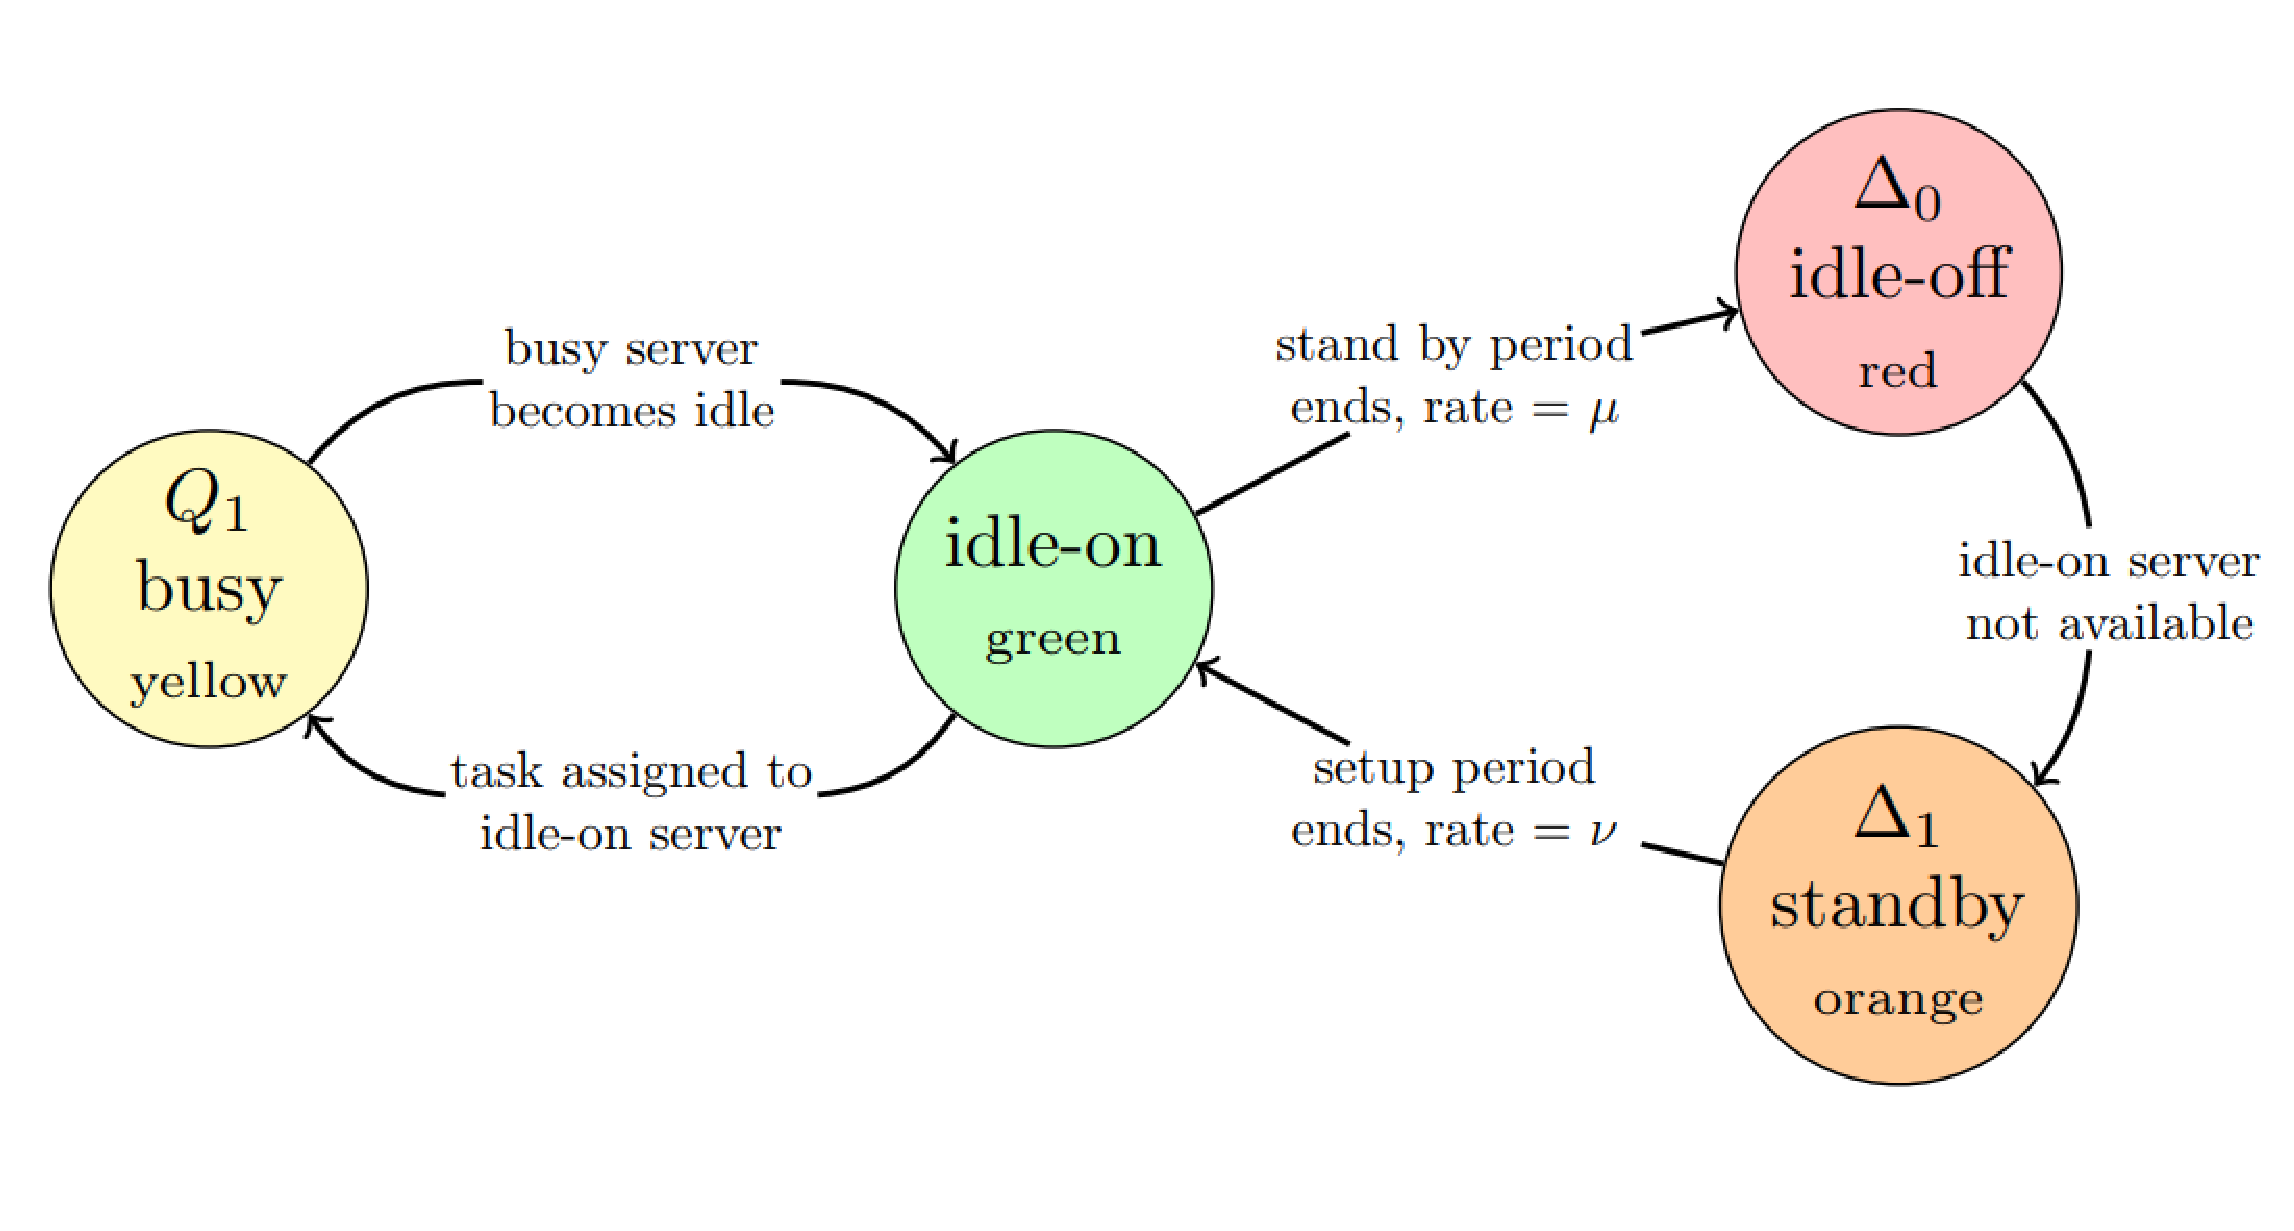
\includegraphics[scale=.3]{tabs}
	\centering
\end{frame}

\begin{frame}{Results}
	For some constant arrival rate $\lambda$ and any $\mu > 0, \nu > 0$, as $N \rightarrow \infty$,
	\begin{enumerate}[label=(\alph*)]
		\item $\E[W^{(N)}] \rightarrow 0$
		\item $\E[Z^{(N)}] \rightarrow 0$
	\end{enumerate}

	\centering
	\textbf{By using the TABS schema, both the mean waiting time and wasted energy vanish in the limit!}
	\centering

\end{frame}

\section{Proofs of TABS Optimality}

\subsection{Notation Overview}

\begin{frame}{Derivation of System State Space}
	\textit{Let:}
	\begin{itemize}
		\item $q_i^{(N)}(t)$ : the fraction of servers with  at least queue length \textit{i} at time \textit{t}
		\item $\Delta_0^{(N)}(t)$ : the fraction of servers in idle-off mode at time \textit{t}
		\item $\Delta_1^{(N)}(t)$ : the fraction of servers in standby mode at time \textit{t}
	\end{itemize}

	\textit{for notational simplicity, let:}
	\begin{itemize}
		\item $q^{(N)}(t) \triangleq (q_i^{(N)}(t)|i = 1,2, \ldots , B)$, and $\delta^{(N)}(t) \triangleq (\delta_0^{(N)}(t),\delta_1^{(N)}(t))$
	\end{itemize}
	\textit{Now define E to be the space of all possible states the system can occupy:}
	\begin{center}
		$E = \{(q,\delta) \in [0,1]^{B+2}\}$
	\end{center}
	\textit{such that:}
	\begin{itemize}\centering
		\item $q_i \geq q_{i+1} \forall i$, and $\delta_0 + \delta_1 + \sum_{i=1}^{B}q_i \leq 1$
	\end{itemize}
\end{frame}

\begin{frame}{ex. 1: System State Space for N = 2, B = 1}
	\begin{itemize}
		\item \textbf{Q: }What are the possible job states in the system at a given time \textit{t}?
		\item \textbf{A: }\{0 jobs, 1 job, 2 jobs\}
		      \begin{center}\centering
			      $q^{(N=2)}(t) = \left\{\frac{0}{2},\frac{1}{2},\frac{2}{2}\right\}$
		      \end{center}
		\item \textbf{Q: }What are the possible server states in the system?
		\item \textbf{A: }\{both servers on, 1 in standby, 1 off\}
		      \begin{center}
			      $\delta_0^{(N=2)}(t) = \delta_1^{(N=2)}(t) = \left\{\frac{0}{2},\frac{1}{2}\right\}$
			      $\delta^{(N=2)}(t) = \left\{(0,0),(0,\frac{1}{2}),(\frac{1}{2},0),(\frac{1}{2},\frac{1}{2}) \right\}$
		      \end{center}

		\item \textbf{Q: }What is E for this scenario?
		\item \textbf{A: }$E$ is all combinations of $q^{(N=2)}(t)$ and $\delta^{(N=2)}(t)$
	\end{itemize}

\end{frame}

\subsection{(3.1) System Behavior as $N \rightarrow \infty$}

\begin{frame}{Deterministic Nature of System as $N \rightarrow \infty$}
	\begin{itemize}
		\item \textbf{Assume that:} $(q^{N}(0),\delta^{N}(0)) $ converges to $(q^{\infty},\delta^{\infty})$
	\end{itemize}
\end{frame}


\subsection{(3.3) Interchange of Limits}

\begin{frame}{Proposition 3.3 : Interchange of Limits}

	\begin{itemize}
		\item Use \texttt{tabular} for basic tables --- see Table~\ref{tab:widgets}, for example.
		\item You can upload a figure (JPEG, PNG or PDF) using the files menu.
		\item To include it in your document, use the \texttt{includegraphics} command (see the comment below in the source code).
	\end{itemize}

	% Commands to include a figure:
	%\begin{figure}
	%\includegraphics[width=\textwidth]{your-figure's-file-name}
	%\caption{\label{fig:your-figure}Caption goes here.}
	%\end{figure}

	\begin{table}
		\centering
		\begin{tabular}{l|r}
			Item    & Quantity \\\hline
			Widgets & 42       \\
			Gadgets & 13
		\end{tabular}
		\caption{\label{tab:widgets}An example table.}
	\end{table}

\end{frame}

\subsection{Mathematics}

\begin{frame}{Readable Mathematics}

	Let $X_1, X_2, \ldots, X_n$ be a sequence of independent and identically distributed random variables with $\text{E}[X_i] = \mu$ and $\text{Var}[X_i] = \sigma^2 < \infty$, and let
	$$S_n = \frac{X_1 + X_2 + \cdots + X_n}{n}
		= \frac{1}{n}\sum_{i}^{n} X_i$$
	denote their mean. Then as $n$ approaches infinity, the random variables $\sqrt{n}(S_n - \mu)$ converge in distribution to a normal $\mathcal{N}(0, \sigma^2)$.

\end{frame}

\end{document}
